\documentclass[letterpaper,10pt]{article}
\usepackage[pdftex]{graphicx}
\usepackage{listings}
\usepackage{alltt}
\usepackage{color}

\definecolor{dkgreen}{rgb}{0,0.6,0}
\definecolor{gray}{rgb}{0.5,0.5,0.5}
\definecolor{mauve}{rgb}{0.58,0,0.82}

\lstset{
	basicstyle=\footnotesize,
	breaklines=true,
}


\begin{document} 

\begin{titlepage}

\begin{center}

\Huge{Assignment 1}

\Large{CS532-s16:  Web Sciences}

\Large{Spring 2016}

\Large{John Berlin}

\Large Generated on \today

\end{center}

\end{titlepage}

\newpage
\noindent
\section*{Question 1}
\begin{verbatim}
Demonstrate that you know how to use "curl" well enough to
correctly POST data to a form.  Show that the HTML response that
is returned is "correct".  That is, the server should take the
arguments you POSTed and build a response accordingly.  Save the
HTML response to a file and then view that file in a browser and
take a screen shot.
\end{verbatim}
\subsection*{Answer}
To post data to form using \verb+curl+ we must first consult the man pages
to see what options are available.
\newline \newline
From the man pages of \verb+curl+:

\begin{alltt}
\emph{-d, --data <data>}
   (puHTTP)  Sends  the  specified data in a \emph{POST request to the HTTP
   server}, in the same way that a browser  does  when  a  user  has
   filled  in an HTML form and presses the submit button. This will
   cause curl to pass the data to the server using the content-type
   application/x-www-form-urlencoded.  Compare to -F, --form.
\end{alltt}
The man pages of \verb+curl+ state it can be used to post data to a form using this syntax:

\begin{lstlisting}[frame=single]
curl -d "formValX=x&formValY=y" http://www.someform.com
\end{lstlisting}
From my recent work with the WS-DL tool mink I believe we can use curl send a uri to WebCite for archival using this command:

\begin{lstlisting}[frame=single]
curl -I -d "url=http://docs.python-requests.org/en/latest/&email=jberlin@cs.odu.edu"  http://webcitation.org/archive
\end{lstlisting}
The curl commands posts and we receive the following response:

\begin{lstlisting}[frame=single]
HTTP/1.1 200 OK
Date: Thu, 28 Jan 2016 01:40:12 GMT
Server: Apache/2.0.63 (Unix) mod_ssl/2.0.63 OpenSSL/0.9.8e-fips-rhel5 mod_auth_passthrough/2.1 mod_bwlimited/1.4 PHP/5.2.9
X-Powered-By: PHP/5.2.9
Content-Length: 5993
Content-Type: text/html
\end{lstlisting}
The form that was used is shown in Figure~\ref{fig:webciteForm}
\begin{figure}
\centering
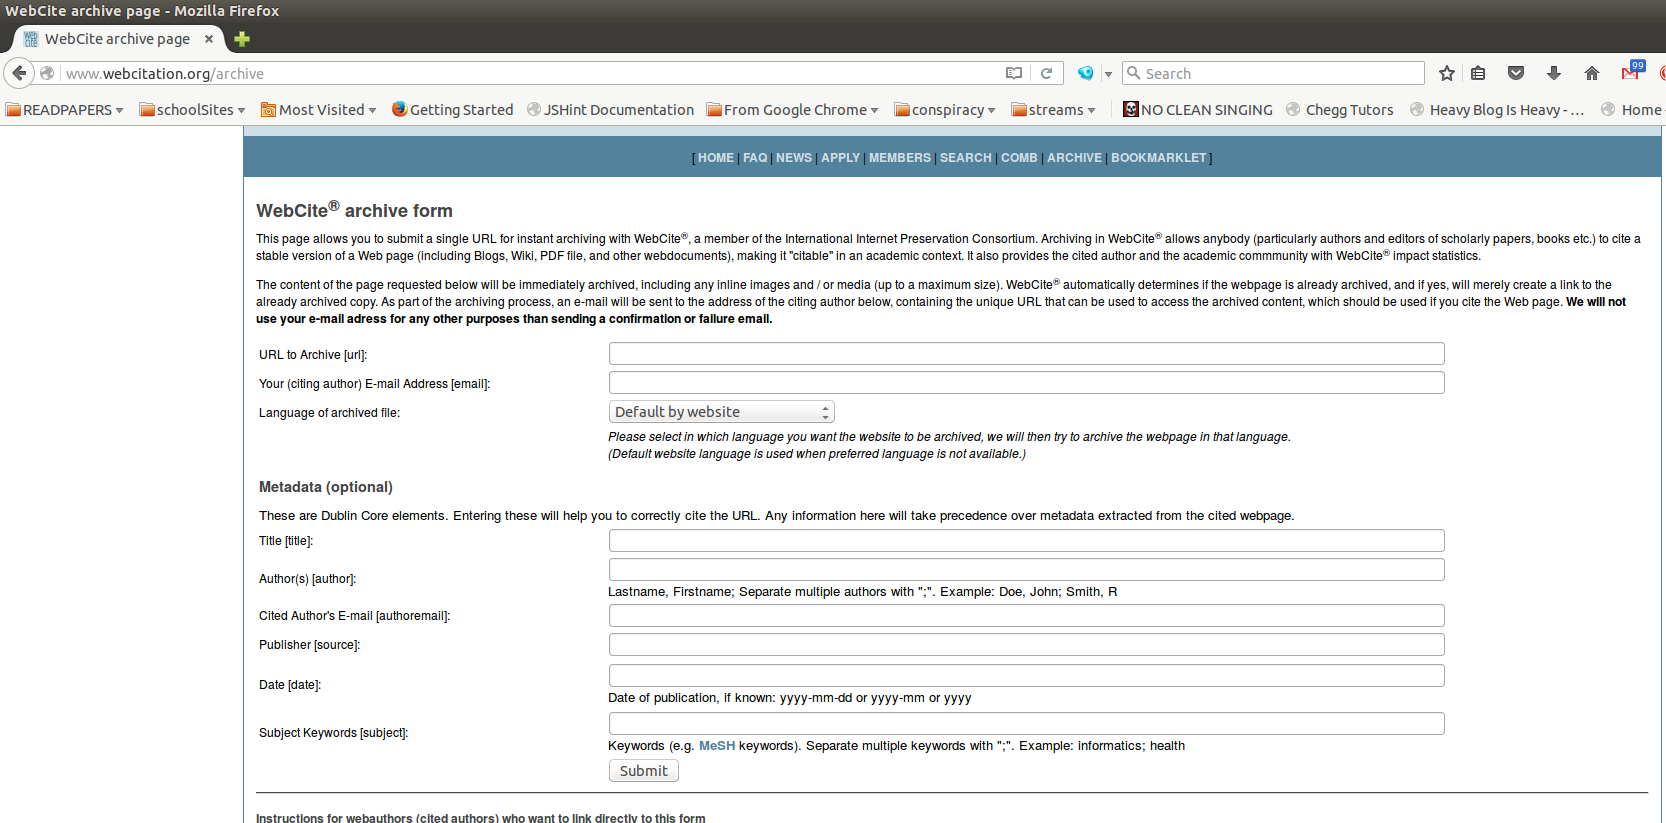
\includegraphics[scale=0.35]{images/webciteForm.png}
\caption{WebCite Archival Form}
\label{fig:webciteForm}
\end{figure}
\newpage
The \verb+-I+ option from the man pages for curl:
\begin{verbatim}
    -I, --head
        (HTTP/FTP/FILE)  Fetch  the HTTP-header only! 
        HTTP-servers feature the command HEAD which this uses to get nothing 
        but the header of a document. When used on an FTP or FILE file, 
        curl displays the file size and last modification time only.
\end{verbatim}
As expected only the headers were returned to in the response. To recive back the html the -I option is removed and curl is executed with these arguments:
\begin{lstlisting}[frame=single]
curl -d "url=http://docs.python-requests.org/en/latest/&email=jberlin@cs.odu.edu"  http://webcitation.org/archive
\end{lstlisting}
\noindent
The rendered html returned by this curl command is shown in Figure~\ref{fig:curled}
\begin{figure}[!ht]
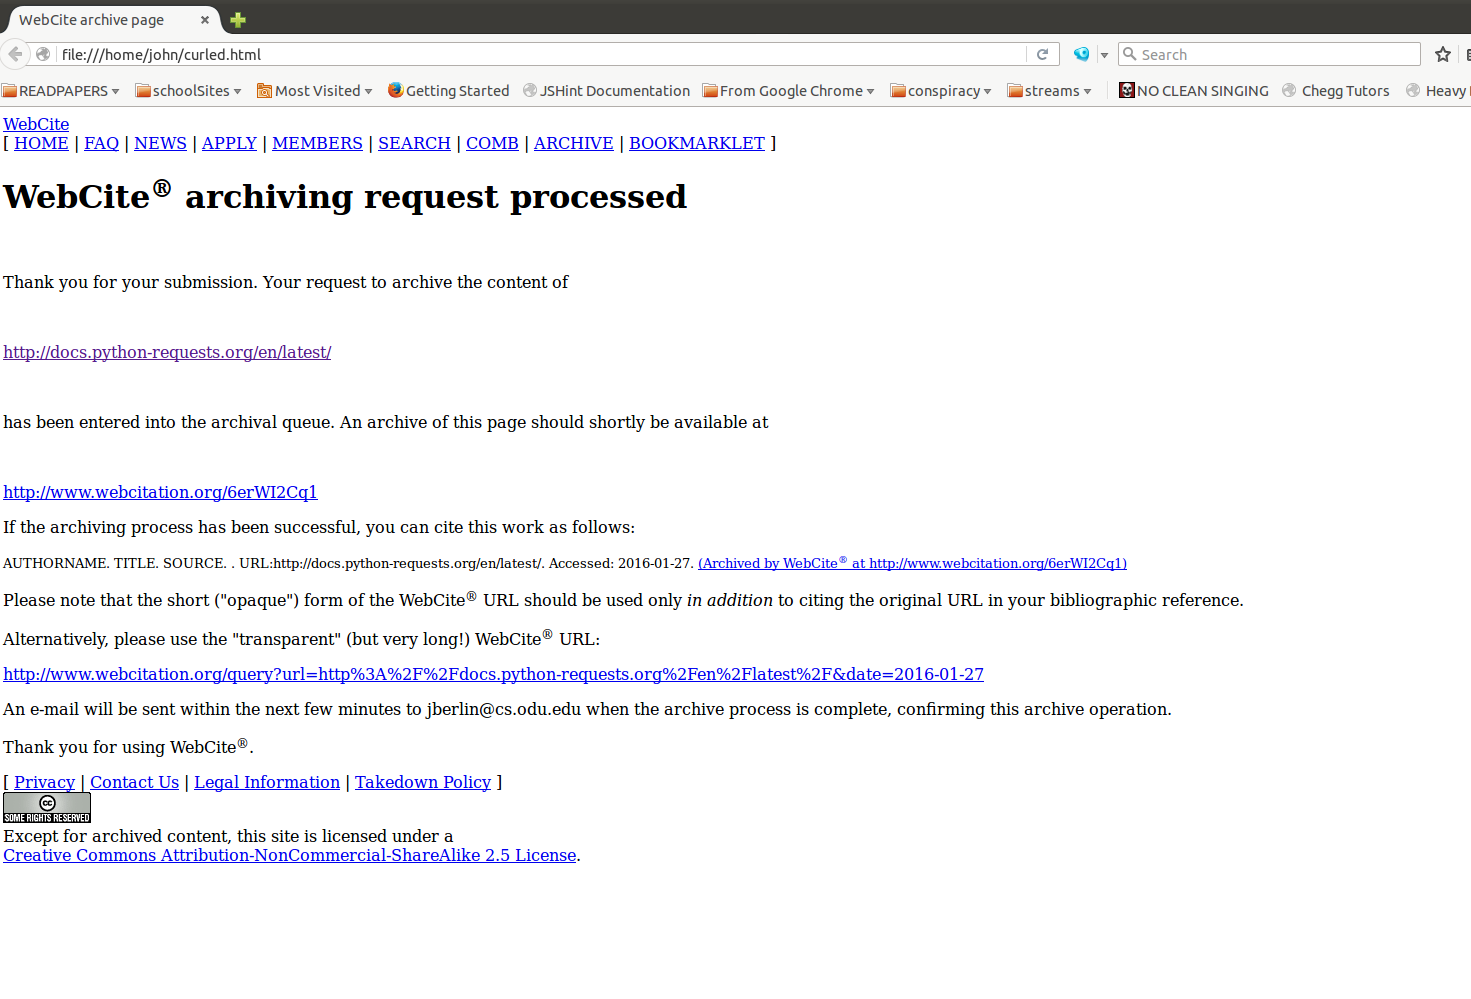
\includegraphics[scale=0.3]{images/curled.png}
\caption{The output of the curl command, rendered in Mozilla Firefox}
\label{fig:curled}
\end{figure}

\newpage
\section*{Question 2}

\begin{verbatim}
Write a Python program that:
  1. takes as a command line argument a web page
  2. extracts all the links from the page
  3. lists all the links that result in PDF files, and prints out
     the bytes for each of the links.  (note: be sure to follow
     all the redirects until the link terminates with a "200 OK".)
  4. show that the program works on 3 different URIs, one of which
     needs to be: 
     http://www.cs.odu.edu/~mln/teaching/cs532-s16/test/pdfs.html
\end{verbatim}
\subsection*{Answer}

\lstinputlisting[language=Python,frame=single,caption={Python program for extracting links from a web page to look for pdf files},label=lst:q2code1,captionpos=b,numbers=left,
numberstyle=\tiny\color{gray},
  keywordstyle=\color{blue},
  commentstyle=\color{dkgreen},
  stringstyle=\color{mauve},showspaces=false,showstringspaces=false,basicstyle=\footnotesize]{followLinks.py}
  
The code is shown in Listing \ref{lst:q2code1} starting on page \pageref{lst:q2code1}:
\begin{itemize}
\item Takes an argument uri specifying the web page to extract links from (line 49)
\item Takes an optional argument to print extra data (line 50)
\item Takes an optional argument to print the headers of all received requests (line 51)
\item Open a session for (line 57), Set our user agent (line 58), Download starting URI (line 70), check to see if won on first uri(line 72), otherwise get all hrefs(line 81), and consume each one in web page informing user if pdf was found(lines 87-120)
\end{itemize}
\noindent
The core libraries used are
\begin{itemize}
\item \textbf{argparse}: I do not like sys.args and closest thing to Commons CLI
\item \textbf{re}: for regular expression support. Do not want some arbitrary href=file.js or malformed uri
\item \textbf{requests}: better urllib, it will handle sneaky redirects automatically   
\item \textbf{bs4}: get the web soup even tho I like my soup hot and sour 
\end{itemize}  
\noindent
\emph{\texttt{strip\_href}} (lines 31 to 44) takes the html text and retrieves all \emph{a} tags and extracts the uri content and adds it the queue. Return the hot soup after extraction.
\newline 

Since requests library handles the redirects for us a check to see if there was some trickery the statement uri != resquest.url checks if the uri found in the extraction is not the same as was the final link. If its not a redirect happened for sure.
\newline
Executing: python3 followLinks.py http://www.cs.odu.edu/~mln/teaching/cs532-s16/test/pdfs.html gives the output
\begin{verbatim}


The link http://www.cs.odu.edu/~mln/pubs/ht-2015/hypertext-2015-temporal-violations.pdf 
	was a link to an actual pdf file  its length is 2184076

The link http://www.cs.odu.edu/~mln/pubs/tpdl-2015/tpdl-2015-annotations.pdf 
	was a link to an actual pdf file  its length is 622981

The link http://arxiv.org/pdf/1512.06195 was a link to an actual pdf file  
	but it was misleading 
		http://arxiv.org/pdf/1512.06195.pdf its length is  1748961

The link http://www.cs.odu.edu/~mln/pubs/tpdl-2015/tpdl-2015-off-topic.pdf 
	was a link to an actual pdf file  its length is 4308768

The link http://www.cs.odu.edu/~mln/pubs/tpdl-2015/tpdl-2015-stories.pdf 
	was a link to an actual pdf file  its length is 1274604

The link http://www.cs.odu.edu/~mln/pubs/tpdl-2015/tpdl-2015-profiling.pdf 
	was a link to an actual pdf file  its length is 639001


The link http://bit.ly/1ZDatNK was a link to an actual pdf file  
	but it was misleading 
	http://www.cs.odu.edu/~mln/pubs/jcdl-2015/jcdl-2015-temporal-intention.pdf 
	its length is  720476

The link http://www.cs.odu.edu/~mln/pubs/jcdl-2015/jcdl-2015-mink.pdf 
	was a link to an actual pdf file  its length is 1254605

The link http://www.cs.odu.edu/~mln/pubs/jcdl-2015/jcdl-2015-arabic-sites.pdf 
	was a link to an actual pdf file  its length is 709420

The link http://www.cs.odu.edu/~mln/pubs/jcdl-2015/jcdl-2015-dictionary.pdf 
	was a link to an actual pdf file  its length is 2350603

\end{verbatim}
\noindent
\newline
Now when executing it with a link straight to a pdf such as http://arxiv.org/pdf/1512.06195.pdf
\begin{verbatim}
The link http://arxiv.org/pdf/1512.06195.pdf 
was a link to an actual pdf file  its length is 1748961
No other links are in a pdf have nice day
\end{verbatim}

\noindent
\newline
For the third and final link I saw one in the full output of the program when running on the required link that looked oddly funky lets try it: http://bit.ly/jcdl-pdf

\begin{verbatim}
Hey were are ok! 200 Done going down the rabit hole 
for http://twitter.com/webscidl

The link 
http://www.cs.odu.edu/~mln/pubs/ht-2015/hypertext-2015-temporal-violations.pdf 
was a link to an actual pdf file  its length is 2184076

The link http://www.cs.odu.edu/~mln/pubs/tpdl-2015/tpdl-2015-annotations.pdf was a link to an actual pdf file  its length is 622981

The link http://arxiv.org/pdf/1512.06195 was a link to an actual pdf file  
	but it was misleading 
	http://arxiv.org/pdf/1512.06195.pdf its length is  1748961

The link http://www.cs.odu.edu/~mln/pubs/tpdl-2015/tpdl-2015-off-topic.pdf was a link to an actual pdf file  its length is 4308768

The link http://www.cs.odu.edu/~mln/pubs/tpdl-2015/tpdl-2015-stories.pdf 
was a link to an actual pdf file  its length is 1274604

The link http://www.cs.odu.edu/~mln/pubs/tpdl-2015/tpdl-2015-profiling.pdf 
was a link to an actual pdf file  its length is 639001


The link http://bit.ly/1ZDatNK was a link to an actual pdf file  
	but it was misleading 
	http://www.cs.odu.edu/~mln/pubs/jcdl-2015/jcdl-2015-temporal-intention.pdf 
	its length is  720476

The link http://www.cs.odu.edu/~mln/pubs/jcdl-2015/jcdl-2015-mink.pdf 
was a link to an actual pdf file  its length is 1254605

The link http://www.cs.odu.edu/~mln/pubs/jcdl-2015/jcdl-2015-arabic-sites.pdf 
was a link to an actual pdf file  its length is 709420

The link http://www.cs.odu.edu/~mln/pubs/jcdl-2015/jcdl-2015-dictionary.pdf 
was a link to an actual pdf file  its length is 2350603

\end{verbatim}

Oddly familiar would you not agree with me. 
\newpage
\section*{Question 3}

\begin{verbatim}
 Consider the "bow-tie" graph in the Broder et al. paper (fig 9):
    http://www9.org/w9cdrom/160/160.html

    Now consider the following graph:

    A --> B
    B --> C
    C --> D
    C --> A
    C --> G
    E --> F
    G --> C
    G --> H
    I --> H
    I --> J
    I --> K
    J --> D 
    L --> D
    M --> A
    M --> N
    N --> D
    O --> A
    P --> G 
    
    For the above graph, give the values for:

    IN: 
    SCC: 
    OUT: 
    Tendrils: 
    Tubes: 
    Disconnected:
\end{verbatim}

\begin{itemize}
\item \textbf{IN}: [M,O,P]  nodes(pages) that can reach the SCC, but cannot be reached from it
\item \textbf{SCC}: [A,B,C,G]  central core, all of whose pages can reach one another along directed links
\item \textbf{OUT}: [D,H]: pages that are accessible from the SCC, but do not link back to it
\item \textbf{Tendrils}: [I,J,K,L] pages that cannot reach the SCC, and cannot be reached from the SCC


\item \textbf{Tubes}: [N]  passage from a portion of IN to a portion of OUT without touching SCC 
  
\item   \textbf{Disconnected}: [E,F] pages who do not fit the descriptions above or has no links to the core or other pages

\end{itemize}

\begin{figure}[!ht]
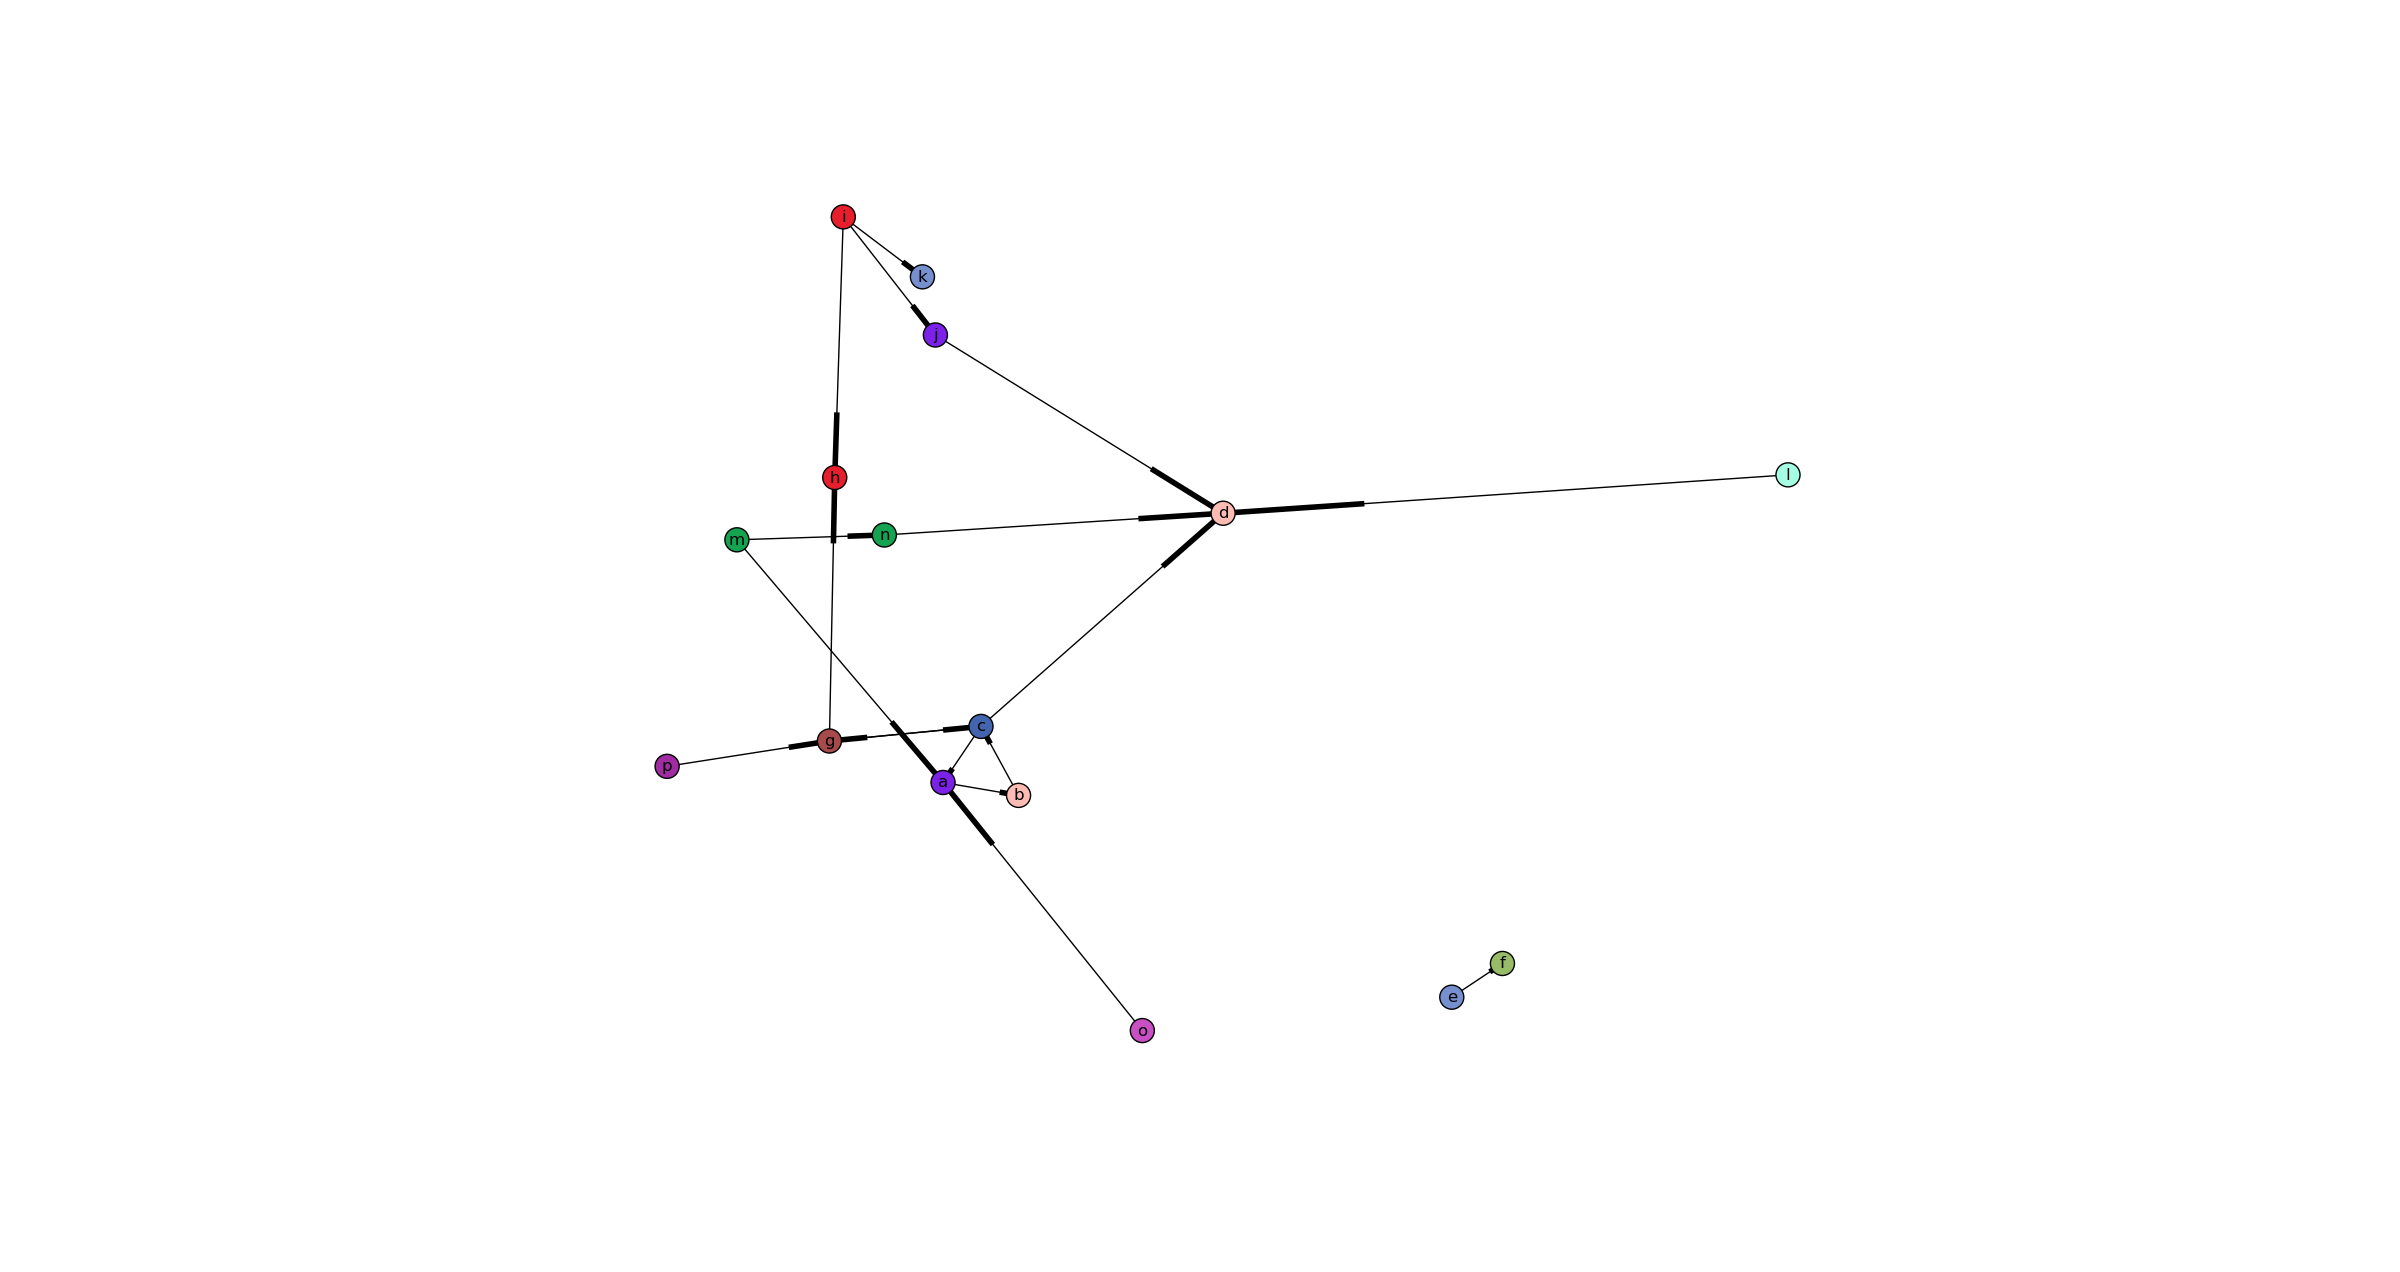
\includegraphics[scale=0.3]{images/bowTie.png}
\caption{A different means of looking at the graph}
\label{fig:bt1}
\end{figure}

\begin{figure}[!ht]
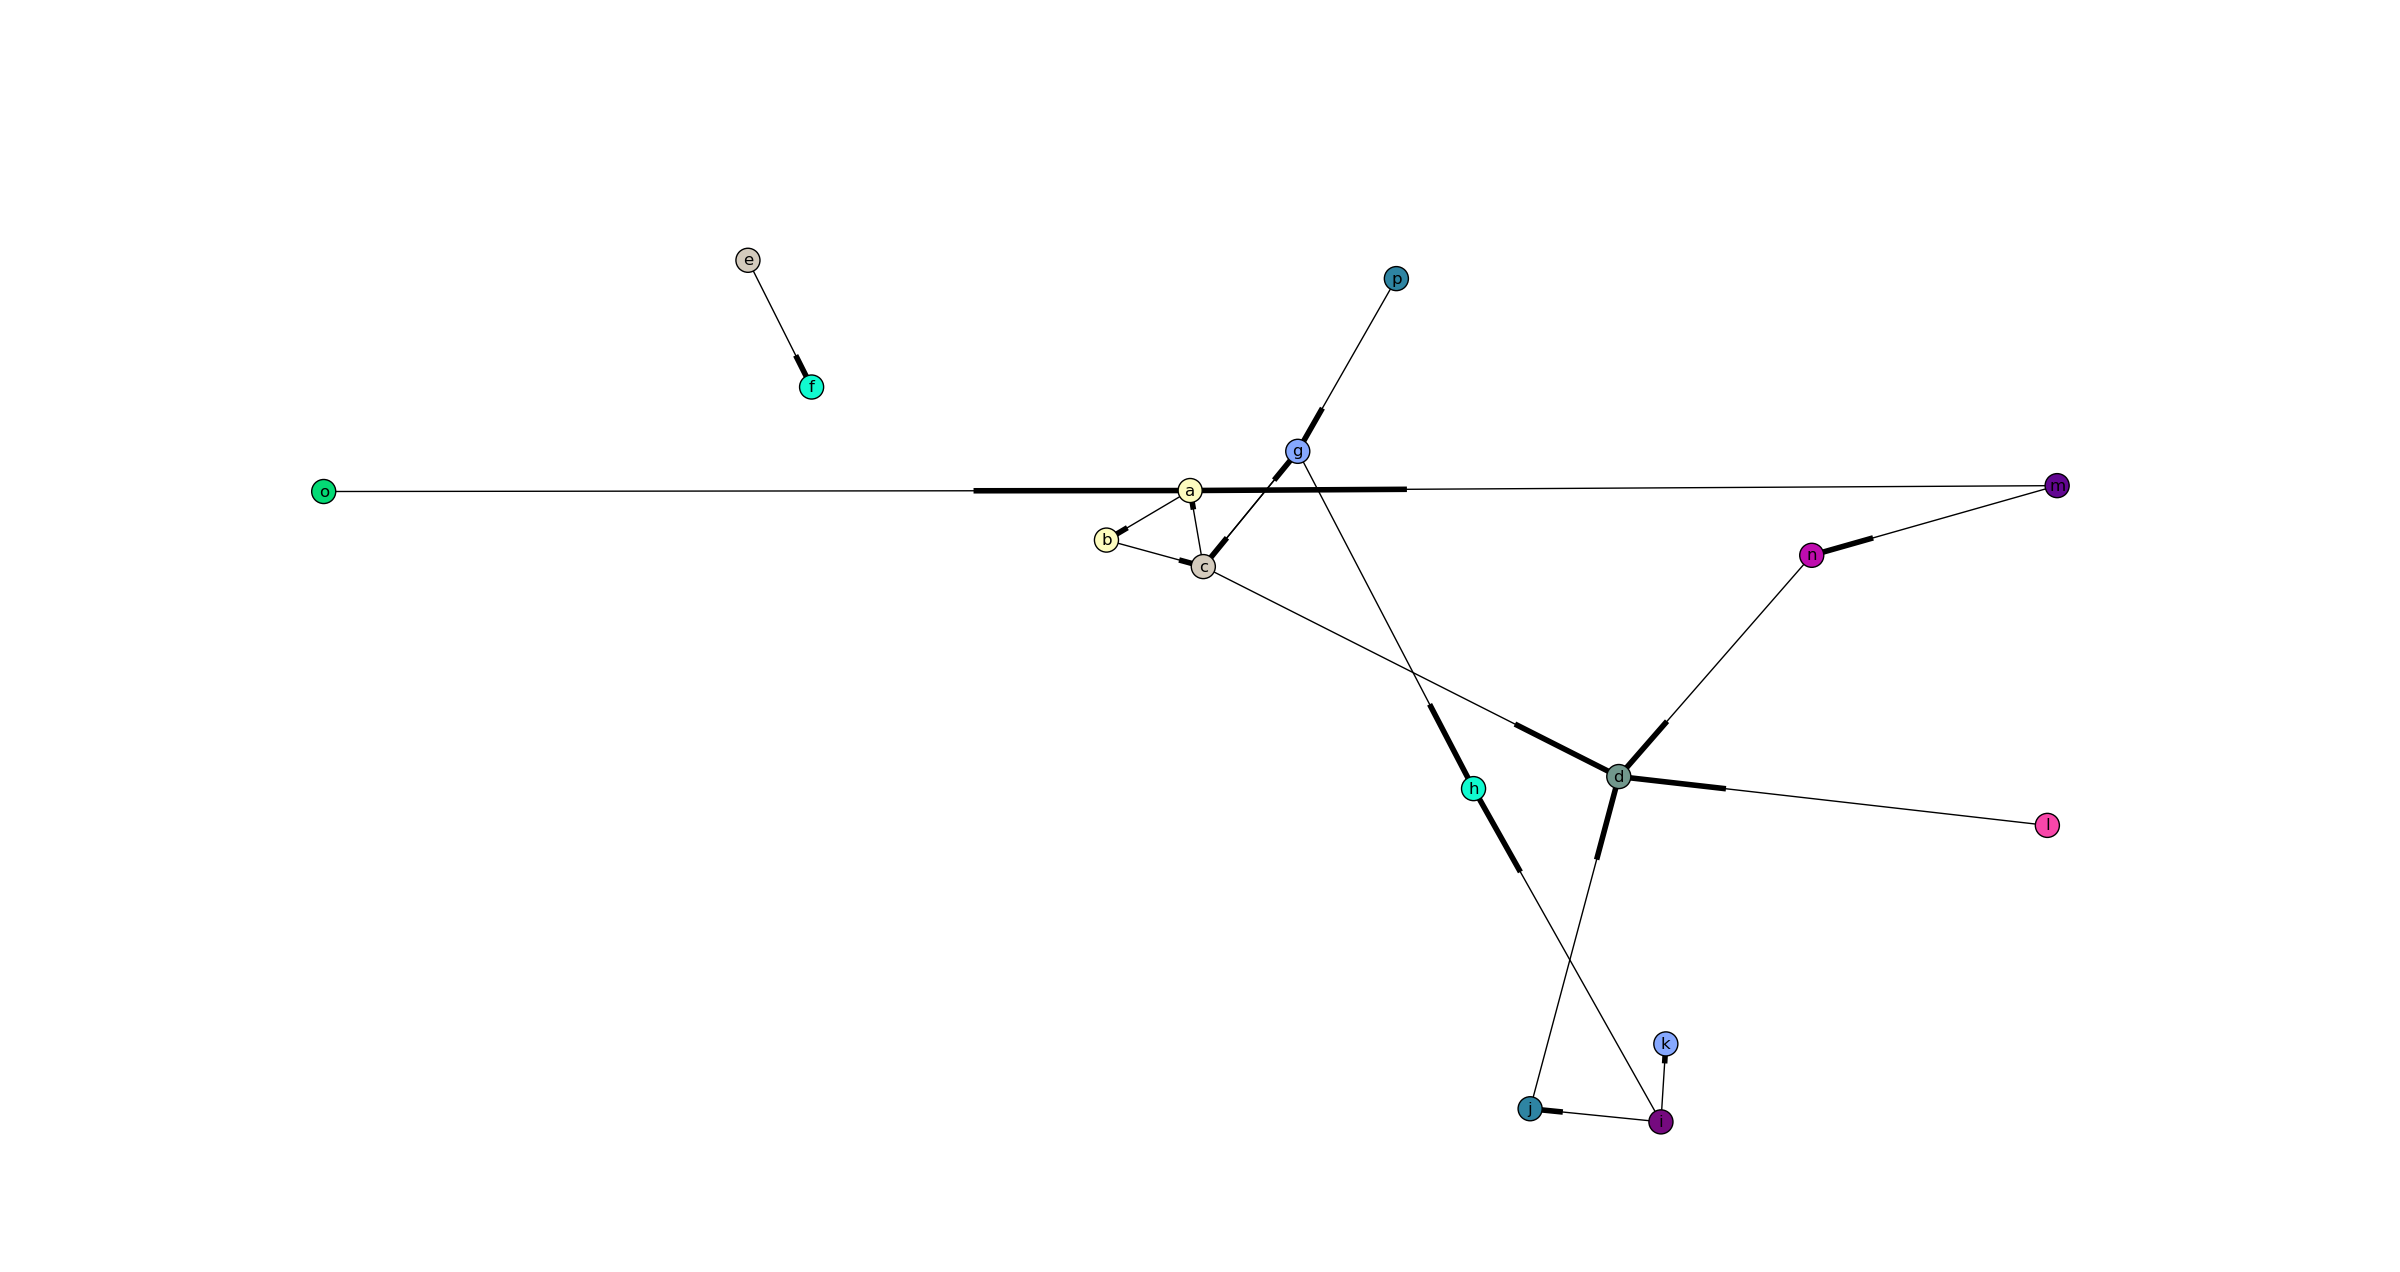
\includegraphics[scale=0.3]{images/bt2.png}
\caption{A different means of looking at the graph2}
\label{fig:bt2}
\end{figure}




\end{document}